\documentclass{standalone}

\usepackage{tikz,amsmath,amssymb,bm,color}
\usetikzlibrary{shapes,arrows,arrows.meta}
% needed for BB
\usetikzlibrary{patterns}
\usetikzlibrary{fit}
\usetikzlibrary{calc,3d}

\pgfdeclareimage[width=1.6cm]{x10}{./matlab/X10.png}
\pgfdeclareimage[width=8mm]{x20}{./matlab/X20.png}
\pgfdeclareimage[width=8mm]{x10d}{./matlab/X10.png}
\pgfdeclareimage[width=4mm]{x20d}{./matlab/X20.png}
%\pgfdeclareimage[width=1.6cm]{x20u}{./matlab/X20.png}
\pgfdeclareimage[width=1.6cm]{x20u}{./matlab/pred.png}


\tikzstyle{FRAME}=[rectangle,draw,ultra thick, minimum width=1.6cm, minimum height=1.6cm,inner sep=0pt]
\tikzstyle{Frame}=[rectangle,draw, ultra thick,minimum width=0.8cm, minimum height=0.8cm,inner sep=0pt]
\tikzstyle{frame}=[rectangle,draw,very thick, minimum width=0.4cm, minimum height=0.4cm,inner sep=0pt]

\definecolor{col10}{rgb}{0,0.5,0.8}%{0.2, 0.5, 1}
\definecolor{col20}{rgb}{0.8,0.2,0.0}%{0.2, 0.5, 1}%{1, 0.2, 0.2}
\definecolor{colLoss}{rgb}{0.8,0.8,0.2}%{0.2, 0.5, 1}%{1, 0.2, 0.2}

\tikzstyle{BOX}=[rectangle,dashed, draw,minimum width=2.1cm, minimum height=0.8cm,inner sep=0pt]
\tikzstyle{LPF}=[rectangle, draw,minimum width=0.8cm, minimum height=0.4cm,inner sep=0pt]
\tikzstyle{DWN}=[rectangle, draw,minimum width=0.4cm, minimum height=0.4cm,inner sep=0pt]
\tikzstyle{CNN}=[rectangle,draw, very thick, minimum width=1.2cm, minimum height=0.6cm,inner sep=0pt]
\tikzstyle{DET}=[rectangle,draw, thick, minimum width=1.2cm, minimum height=0.6cm,inner sep=1pt]


\tikzstyle{Loss}=[circle, fill=colLoss, very thick,draw, minimum size=0.8cm, inner sep=0pt]
\tikzstyle{SUM}=[circle, thick,draw, minimum size=0.3cm, inner sep=0pt]
\tikzstyle{arr}=[thick, -stealth]


\begin{document}

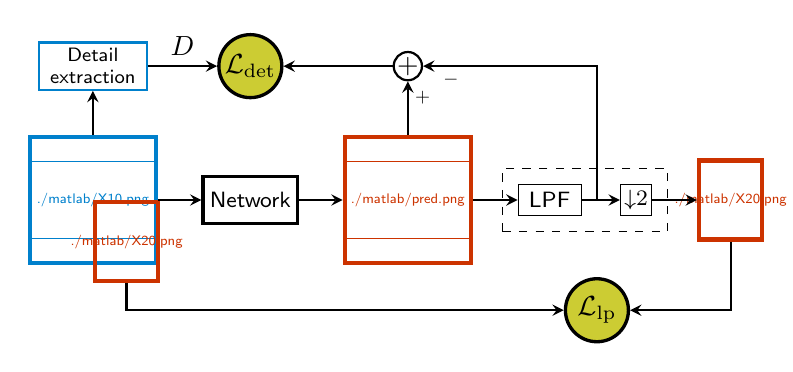
\begin{tikzpicture}[node distance=2cm]
\sf

\node[coordinate](O) at (0,0){}; % origine
\node[FRAME,col10](I1) at (0,0){\pgfuseimage{x10}}; 
\node[Frame,col20,anchor=north west](I2) at (0,0){\pgfuseimage{x20}}; 

\node[CNN, right of=I1,font=\footnotesize,xshift=-0mm](net) {Network};

\node[FRAME,col20,right of=net, xshift=-0mm](pred) {\pgfuseimage{x20u}}; 

\node[LPF, right of=pred,font=\footnotesize,xshift=-2mm](lpf) {LPF};
\node[DWN, right of=lpf, node distance = 1.1cm,font=\footnotesize](down) {${\downarrow}2$};
\node[BOX, right of=pred,xshift = 2.5mm,font=\footnotesize](Down) {};

\node[Frame,col20,right of = down,xshift=-8mm](predScaled) {\pgfuseimage{x20}};

\draw[arr] (I1)--(net);  \draw[arr] (net)--(pred); \draw[arr] (pred)--(lpf);
 \draw[arr] (lpf)--node[coordinate,pos=0.4](pt){}(down); \draw[arr] (down)--(predScaled); 

\node[Loss,draw, below of=pt, node distance = 1.4cm](loss) {$\mathcal{L}_{\rm lp}$};

\draw[arr] (I2)|-(loss);
\draw[arr] (predScaled)|-(loss);

% NEW BRANCH

\node[Loss,draw, above of=net, node distance = 1.7cm](lossDet) {$\mathcal{L}_{\rm det}$};

\node[DET, above of=I1, node distance = 1.7cm, font=\scriptsize,draw=col10](det) {\parbox{1.3cm}{\centering Detail extraction}};

\node[SUM, above of=pred, node distance = 1.7cm](sum){$+$};

\draw[arr] (I1)--(det);
\draw[arr] (det)--node[above]{$D$}(lossDet);
\draw[arr] (pred)--node[pos=0.7,right,scale=0.7]{$+$}(sum);
\draw[arr] (pt)|-node[pos=.92,scale=0.7,below]{$-$}(sum);
\draw[arr] (sum)--(lossDet);




\end{tikzpicture}

\end{document}